\bluepage{Shaders and Shader Programs}

\begin{frame}\frametitle{Two languages are needed / jsou potřeba dva jazyky}
\scriptsize
\begin{itemize}
  \item OpenGL standard describes API and OpenGL shading language -- GLSL.
  \item GLSL describes structure of programs running on GPU.
  \item Programmer needs to write the code in two languages -- one for CPU and one for GPU.
\end{itemize}

\begin{itemize}
  \item OpenGL standard popisuje i jazyk GLSL.
  \item Jazyk GLSL popisuje programy, které běží na GPU.
  \item Programátor 3D grafiky píše aplikaci vždy ve 2 jazycích.
\end{itemize}
  \begin{figure}[h]
    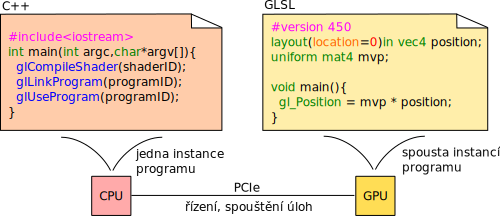
\includegraphics[width=10cm,keepaspectratio]{pics/program/cpp_and_glsl.pdf}
  \end{figure}
\end{frame}

\begin{frame}\frametitle{Shader programs, Shaders}
\scriptsize
\begin{itemize}
\item A shader program is program that runs on GPU.
\item Shader Program is composed of few stages called shaders.
\item There are six shader types: \textbf{vertex}, \textbf{fragment}, geometry, tesselation control, tesselation evaluation and compute shader.
\item Shader program does not have to contain all stages.
\item Stages can be shared among multiple programs.
\item Shaders can be precompiled or compiled in runtime.
\item Shader programs are linked.
\end{itemize}

\begin{itemize}
\item Program, který běží na GPU se v OpenGL označuje jako shader program.
\item Shader Program je složen z několika částí (stages), které se nazývají shader.
\item Existuje 6 typů shaderů: \textbf{vertex}, \textbf{fragment}, geometry, tesselation control, tesselation evaluation a compute shader.
\item Program nemusí obsahovat všechny typy shaderů.
\item Jednotlivé shadery lze sdílet mezi vícero programy.
\item Shadery se kompilují (za běhu aplikace).
\item Programy se linkují (za běhu aplikace), ale mohou být předpřipraveny v binárce.
\end{itemize}
\end{frame}

\begin{frame}\frametitle{Shader combinations / Kombinace shaderů v programu}
  Valid and commonly used shader combinations:\\
  Validní a často používané kombinace shaderů:
  \begin{figure}[h]
    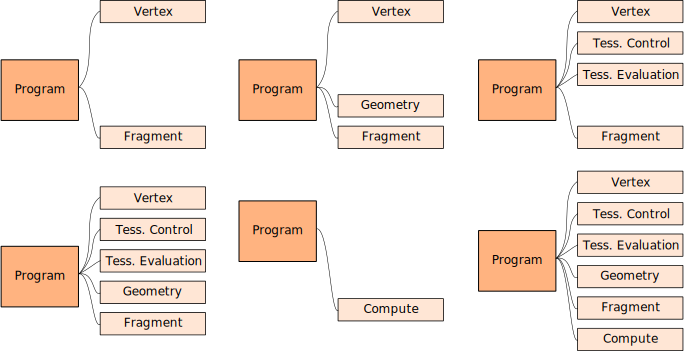
\includegraphics[width=10cm,keepaspectratio]{pics/program/shader_combination.pdf}
  \end{figure}
\end{frame}

\begin{frame}[fragile]\frametitle{Shader compilation / Kompilace shaderů}\scriptsize
\begin{minted}[bgcolor=bg]{packages/c_cpp.py:CppLexer -x}
GLuint createShader(GLuint type, std::string const& src) {
  //create handle
  GLuint id = glCreateShader(type);

  //set shader source
  char const* vsSrc[1] = {
    src.c_str()
  };
  glShaderSource(id, 1, vsSrc, nullptr); 

  //compile shader
  glCompileShader(id);

  //get compilation status
  int compileStatus;
  glGetShaderiv(id, GL_COMPILE_STATUS, &compileStatus);
  if (compileStatus != GL_TRUE) {
    //get message info length
    GLint msgLen;
    glGetShaderiv(id,GL_INFO_LOG_LENGTH,&msgLen);
    auto message = std::string(msgLen,' ');
    // get message
    glGetShaderInfoLog(id, msgLen, nullptr, message.data());
    std::cerr << message << std::endl;
  }
  return id;
}
\end{minted}
\end{frame}

\begin{frame}[fragile]\frametitle{Program linking}\scriptsize
\begin{minted}[bgcolor=bg]{packages/c_cpp.py:CppLexer -x}
GLuint createProgram(std::vector<GLuint>const& shaders) {
  //create handle
  GLuint prg = glCreateProgram();

  //attach shaders
  for(auto const&shader:shaders)
    glAttachShader(prg,shader);

  //link program
  glLinkProgram(prg);

  //get link status
  GLint linkStatus;
  glGetProgramiv(prg, GL_LINK_STATUS, &linkStatus);
  if(linkStatus != GL_TRUE){
    //get message info length
    GLint msgLen;
    glGetProgramiv(prg,GL_INFO_LOG_LENGTH,&msgLen);
    auto message = std::string(msgLen,' ');
    glGetProgramInfoLog(prg, msgLen, nullptr, message.data());
    std::cerr << message << std::endl;
  }
  return prg;
}
\end{minted}
\end{frame}

\begin{frame}[fragile]\frametitle{1 Triangle example / ukázka jednoho trojúhelníku}\scriptsize
\begin{minted}[bgcolor=bg]{packages/c_cpp.py:CppLexer -x}

int main(int32_t argc,char*argv[]){
  ...
  // vertex shader source
  auto vsSrc = R".(
  #version 460
  void main(){
    gl_Position=vec4(gl_VertexID&1,gl_VertexID>>1,0,1);
  }
  ).";

  // fragment shader source
  auto fsSrc = R".(
  #version 460
  out vec4 fColor;
  void main(){
    fColor = vec4(1);
  }
  ).";

  GLuint vs = compileShader(GL_VERTEX_SHADER  ,vsSrc);
  GLuint fs = compileShader(GL_FRAGMENT_SHADER,fsSrc);
  GLuint program = createProgram({vs,fs});
}
\end{minted}
\end{frame}


